\documentclass[11pt]{article}
\usepackage[margin=1.05in]{geometry}
\usepackage{amsmath,amssymb}
\usepackage{graphicx}
\usepackage{booktabs}
\usepackage{xcolor}
\usepackage[colorlinks=true,linkcolor=blue!50!black,urlcolor=blue!50!black]{hyperref}
\usepackage{parskip}
\usepackage{float}

\newcommand{\g}{\textsf{g57}}
\newcommand{\fmix}{\texttt{fmix}}
\newcommand{\X}{\mathrm{X}}

\title{The Split Stage of Phase B:\\
\large the split twist, its instrumentation, and the bracket-draw calibration}
\author{local-mixing project}
\date{2026-08-05}

\begin{document}
\maketitle

\begin{abstract}
Phase B's job, under the 2026-08-04 reframe, is to \emph{break the \g\ structure}
of a phase-A output --- anti-inversion with absolute spread --- rather than to mix
state. We partition phase B in two parts and report the first part, now shipped:
a \emph{split stage} in which a single move --- the \emph{split twist} --- splits
every \g\ into a (CNOT/NCNOT, 2-control AND) pair while carrying long-range
\emph{absorbed} pure-NOT twists and one cross per split. The stage runs to \g\
exhaustion. On five inputs (99k--1.66M gates, 5--99\% \g) it eliminates every
complemented gate at a measured growth of $1{+}$(comp fraction) ($\times1.7$--$2.0$),
in seconds to minutes, with every rewrite locally verified and the full circuit
functionally checked. Wire canaries show twist coverage is absolute across the
circuit with only the geometric end effect. A three-arm A/B over the bracket draw
fixed both pathologies found on the way: the original other-half-first cascade
drifted to near-full-circuit spans (midpoint crossing a constant 100\%), and a
na\"ive own-direction draw produced a 28\% spike of near-zero spans. The shipped
rule --- twist side drawn proportionally to the circuit length remaining on that
side, bracket = farthest of $k{=}2$ samples --- lands mean span $0.57$ of the
circuit, midpoint crossing 71\%, and a 0--5\% span mass of 2.9\%.
\end{abstract}

\section{Context and goal}

A phase-A output is a \g-dominated circuit: complemented two-control gates
$a \mathbin{\oplus\!=} \lnot(\ell_b \wedge \ell_c)$ plus X-series conjunction
gates. The \g\ population is exactly the structure an inverter can lean on, so
phase B opens by destroying it: every \g\ must be re-spelled as ordinary
conjunction material, and the re-spelling must not be locally explicable ---
the compensation for each local rewrite should live far away in the circuit.
Phase B is therefore split in two: \textbf{part 1} (this report) breaks the
structure; \textbf{part 2} is the existing phase-B menu, starting from the
broken form.

\section{The move}

\subsection{The split}
One split-twist move picks a uniformly random \g\ $g$ with target $w$ and
splits it by the randomized first-failing-literal presplit (the literal
shuffle is the design's $r$ bit). For the canonical two-control \g,
$g:\; a \mathbin{\oplus\!=} (b \vee \lnot c)$ becomes either
$\{a \mathbin{\oplus\!=} b,\; a \mathbin{\oplus\!=} \lnot b\lnot c\}$ or
$\{a \mathbin{\oplus\!=} \lnot c,\; a \mathbin{\oplus\!=} bc\}$:
a single-control gate $g_1$ and a two-control AND $g_2$, exact and disjointly
fired. Pieces stay in place (no birth transport --- $g_1$ must sit where the
bracket forms; $g_2$'s transport is the move's closing cross), inherit origin
and litter with a fresh event, and take \emph{opposite directions} from a fair
draw. That sibling convention is now global: every \g\ presplit anywhere in
\fmix\ gives its pieces alternating directions (the old independent
per-piece law was a bug; pre-2026-08-05 walks do not replay).

\subsection{The absorbed pure-NOT twist}
With probability \texttt{p\_join} the split carries a twist on wire $w$.
Two facts make it free:
\begin{enumerate}
\item a gate targeting $w$ never reads $w$, so it \emph{commutes} with $\X(w)$;
\item composing $\X(w)$ into a 1-control gate targeting $w$ \emph{is} that gate
with its control polarity flipped:
$(w \mathbin{\oplus\!=} \ell(b)) \cdot (w \mathbin{\oplus\!=} 1) =
 (w \mathbin{\oplus\!=} \lnot\ell(b))$ --- CNOT $\leftrightarrow$ NCNOT, one gate.
\end{enumerate}
So for brackets $g_1 \dots h_1$ both targeting $w$, at any distance:
\[
g_1^\flat \cdot S' \cdot h_1^\flat
\;=\; g_1 \cdot \X(w) \cdot S' \cdot \X(w) \cdot h_1
\;=\; g_1 \cdot S \cdot h_1,
\]
where $\flat$ flips the bracket's control polarity and $S'$ flips the polarity
of every \emph{$w$-reading} pin in the open segment (gates targeting $w$ are
invariant). The function is preserved with \textbf{zero synthetic gates} ---
strictly better than the retired free-standing NEG twist, which paid two X
gates and needed a bracket-cancel tabu. This is the pure-NEG twist revived in
absorbed form. The anti-inversion effect is the point: after absorption,
$\{g_1^\flat, g_2\}$ no longer XOR to $g$ locally --- the compensation lives at
$h_1^\flat$ and in the flipped segment, typically across a large fraction of
the circuit.

The other bracket comes from the population of gates targeting $w$: a \g\
(split on selection, its 1-control piece absorbs) or a CNOT/NCNOT (absorbs
directly). Segment \g s that \emph{read} $w$ are force-split before their
pins flip (5a). That is not needed for correctness --- a polarity flip inside a
complemented conjunction is exact --- but it preserves the \g{}+X-series
closure part 2 relies on, and it is the stage's main engine: a long twist
retires every $w$-reading \g\ on its path.

\subsection{The cross}
The move closes with one ordinary cross shot from $g_2$ (it runs whether or
not the twist landed, but not when the \texttt{p\_join} coin ends the move
early). Transport of the AND pieces is thus the cross machinery's job, under
its normal counters and undo journal.

\subsection{Layer embedding and exits}
At layer 1 the split twist is a third dispatch in the twist slot
(\texttt{p\_split\_twist}). At layer 2, \texttt{--split} arms the stage: the
split twist is the \emph{only} move running (no brake, overlay, shuffle, DB,
or thermostat) until either \textbf{exit A} --- no \g\ remains anywhere (in
practice always this one) --- or \textbf{exit B} --- \texttt{--split-fail-limit}
consecutive bracket failures. The boundary pins the live split-twist dispatch
to zero and releases the round to the command line's phase-B parameters;
\texttt{--split-stop} ends the run there instead (trial mode). The stage
phase persists in the state file as a tri-state (never armed / live / ended),
so resumes continue, never silently restart, and warn when a live stage is
resumed without \texttt{--split}. State files are v2; v1 files load, old
binaries refuse v2.

\section{Instrumentation}

\textbf{Counters.} \texttt{prims} (the picked \g), \texttt{hspl} (bracket
splits), \texttt{segs} (segment splits), \texttt{joins}, \texttt{fails},
\texttt{xmid} (brackets straddling the midpoint), span sum + a 5\%-bucket
span histogram; a per-move \texttt{split} line carries all of them plus the
move's span.

\textbf{Wire canaries} (\texttt{--split-canaries}, default 256). A canary
sits on a wire immediately right of an anchor gate, planted uniformly at
stage start, remembering its \emph{original} position. A twist whose bracket
span covers it on its wire complements the value carried there --- one flip.
Canaries ride the material: on anchor death they re-anchor to the live left
neighbor (the eviction must run \emph{after} the prior partner's unlink when
both partners of a splice die --- the one real bug the adversarial review
caught, along with resume tri-state semantics and exit gating, all fixed and
re-verified). The flips-by-original-position profile is the stage's
spread/reach deliverable.

\textbf{Rank stamps.} Positions and sides come from an $O(n)$ rank restamp
every 8192 moves \emph{and} on $>25\%$ growth. Ranks are heuristics
(selection, \texttt{xmid}, canary positions); correctness never depends on
them --- the segment itself is found by an alternating bidirectional walk.

\section{Trials}

Five inputs, all runs \texttt{--split --split-stop}, local verification on
every rewrite, global functional checks at the boundary; every run ended by
exit A with the failure limit untouched.

\begin{center}
\small
\begin{tabular}{lrrrrrr}
\toprule
input & gates & \g\ frac & moves & end size & growth & time \\
\midrule
gadgetized n128 & 99{,}016 & 5.2\% & 1{,}462 & 106{,}000 & $\times$1.07 & 1.5s \\
cg1 slow-anneal & 1{,}020{,}340 & 69.2\% & 5{,}495 & 1{,}731{,}515 & $\times$1.70 & 129s \\
cg1 fast-anneal & 1{,}016{,}535 & 16.1\% & 3{,}788 & 1{,}184{,}051 & $\times$1.16 & 74s \\
cg1\_phaseA5 ($p_{\rm join}{=}1$) & 64{,}782 & 73.5\% & 2{,}713 & 115{,}629 & $\times$1.78 & 4s \\
g57A phaseA ($p_{\rm join}{=}1$) & 1{,}664{,}636 & 83.5\% & 4{,}818 & 3{,}060{,}082 & $\times$1.84 & 293s \\
nR20\_mixed ($p_{\rm join}{=}1$) & 179{,}132 & 99.3\% & 5{,}357 & 362{,}995 & $\times$2.03 & 27s \\
\bottomrule
\end{tabular}
\end{center}

Three regularities, all predicted by the design:
\textbf{(i) growth $\approx 1 +$ comp fraction} --- the pair split \emph{is}
the growth; cross ladders are net noise.
\textbf{(ii) segment splits dominate}: $\sim$99\% of \g\ depletion arrives
through 5a --- the stage is a few thousand large sweeps, not a per-gate crawl.
\textbf{(iii) brackets never starve}: every split mints a permanent 1-control
bracket, so failures stay near zero and exit is always by exhaustion.

\textbf{Gate makeup.} The cleanest case, \texttt{nR20\_mixed} (99.3\% true
\g, no 1-control gates at all on input) exits as: CNOT 24.6\% / NCNOT 24.6\%
(dead-even --- the polarity churn of the absorbed NOTs), 2-control ANDs at a
$1{:}2{:}1$ negation-count ratio (the binomial signature of the presplit
composed with uniform polarity churn), a $\sim$2\% cross-ladder tail, zero
comp. X gates pass through untouched in absolute count on every input.

\section{Coverage: the canaries}

\begin{figure}[H]
\centering
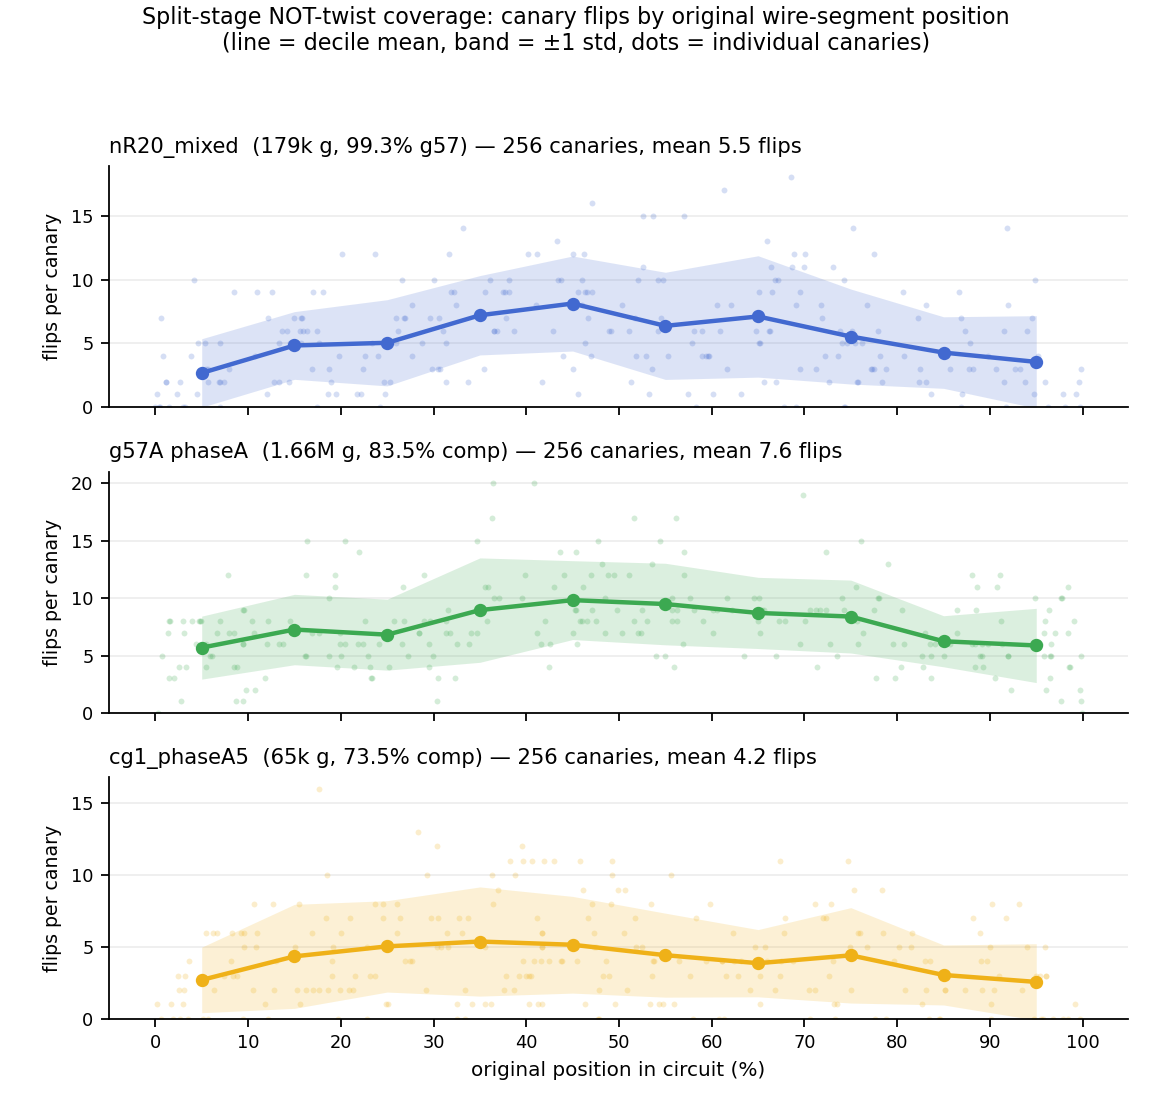
\includegraphics[width=0.92\textwidth]{../reports/split_trials_20260805/canary_flips_by_position.png}
\caption{Flips per canary by \emph{original} position: decile mean (line),
$\pm1$ std (band), individual canaries (dots); the three $p_{\rm join}{=}1$
phase-A runs. A broad mid-circuit plateau at roughly $2\times$ the edge
coverage --- the $2x(1{-}x)$ geometry of a span between two near-uniform
endpoints --- with no asymmetry and no origin clustering. Std $\approx$ mean:
spans are few and long, so per-canary counts are overdispersed.}
\end{figure}

Reach is absolute up to the unavoidable end effect. If flatter \emph{edge}
coverage is ever wanted, the lever is biasing bracket choice toward the ends,
not more twists.

\section{Calibrating the bracket draw}

The original draw was a cascade: prefer a \g\ in the \emph{other half} of the
circuit, then a CNOT there, then the same-half classes. It worked --- but
\texttt{xmid} sat at a constant 100\%: an other-half bracket essentially
always exists, so the midpoint-crossing counter was a target, not a
measurement, and an overshoot. Two redesign steps, measured on
\texttt{nR20\_mixed} at equal seed (Figure~\ref{fig:spans}):

\begin{figure}[H]
\centering
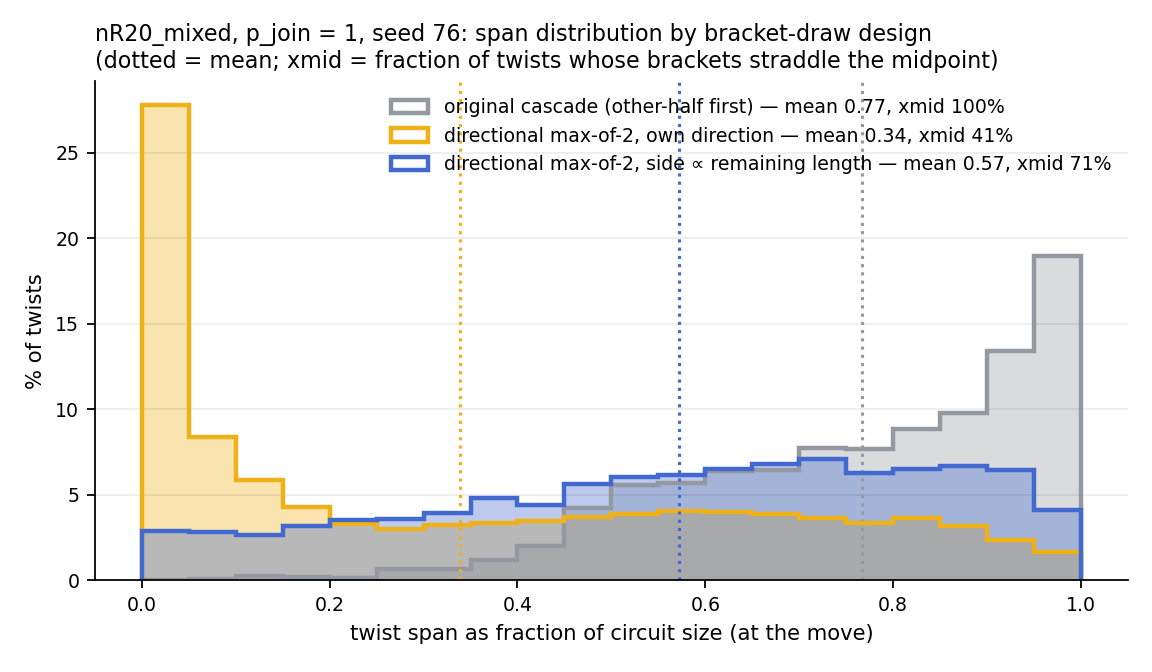
\includegraphics[width=0.9\textwidth]{../reports/split_trials_20260805/span_compare_nR20.png}
\caption{Twist span as a fraction of the circuit, three bracket-draw designs
on \texttt{nR20\_mixed} ($p_{\rm join}{=}1$, same seed).}
\label{fig:spans}
\end{figure}

\begin{center}
\small
\begin{tabular}{lrrrrr}
\toprule
arm & mean span & 0--5\% mass & xmid & fails & moves \\
\midrule
other-half cascade ($k{=}0$) & 0.77 & 0.03\% & 100\% & 0 & 3{,}811 \\
own-direction, max-of-2 & 0.34 & 27.8\% & 41\% & 137 & 6{,}417 \\
\textbf{side $\propto$ length, max-of-2 (shipped)} & \textbf{0.57} & \textbf{2.9\%} & \textbf{71\%} & 1 & 5{,}357 \\
\bottomrule
\end{tabular}
\end{center}

\textbf{The cascade drifts long.} Its spans are far longer than uniform
other-half placement predicts (mode 95--100\%). The histogram exposed a
feedback loop: segment sweeps clear the middle first, surviving \g s cluster
at the edges, and edge-picked primaries paired with other-half brackets span
nearly the whole circuit --- self-reinforcing as the stage proceeds.

\textbf{Own-direction spikes short.} Restricting candidates to the picked
\g's own stored direction and taking the farthest of $k{=}2$ uniform samples
lands the design mean ($\tfrac23 \cdot \mathbb{E}[\text{available run}]
\approx 0.34$) --- but 28\% of twists fall in the 0--5\% bucket: primaries
picked near the edge their direction points at have almost no run to use.

\textbf{Shipped: side drawn $\propto$ remaining length.} The twist side is
drawn with probability proportional to the circuit length remaining on it, so
a side is picked exactly as rarely as it is short --- a tiny span now needs a
short side \emph{and} the coin to pick it (squared suppression). The 0--5\%
mass collapses to 2.9\%, the mean lands at 0.57 (above the na\"ive $4/9$
because edge-clustered survivors are sent sweeping across the circuit),
midpoint crossing settles at an honest 71\%, failures essentially vanish, and
the canaries confirm the coverage read (Figure~\ref{fig:armcanaries}): the
shipped draw has the highest mean coverage (6.4 flips/canary) and the best
edge coverage of the three arms. The knob \texttt{--split-reach-k} remains
the length-bias dial ($1$ = uniform on the drawn side, $2 \approx \tfrac23$
of the run, $3 \approx \tfrac34$; $0$ = the legacy cascade, kept as an A/B
arm).

\begin{figure}[H]
\centering
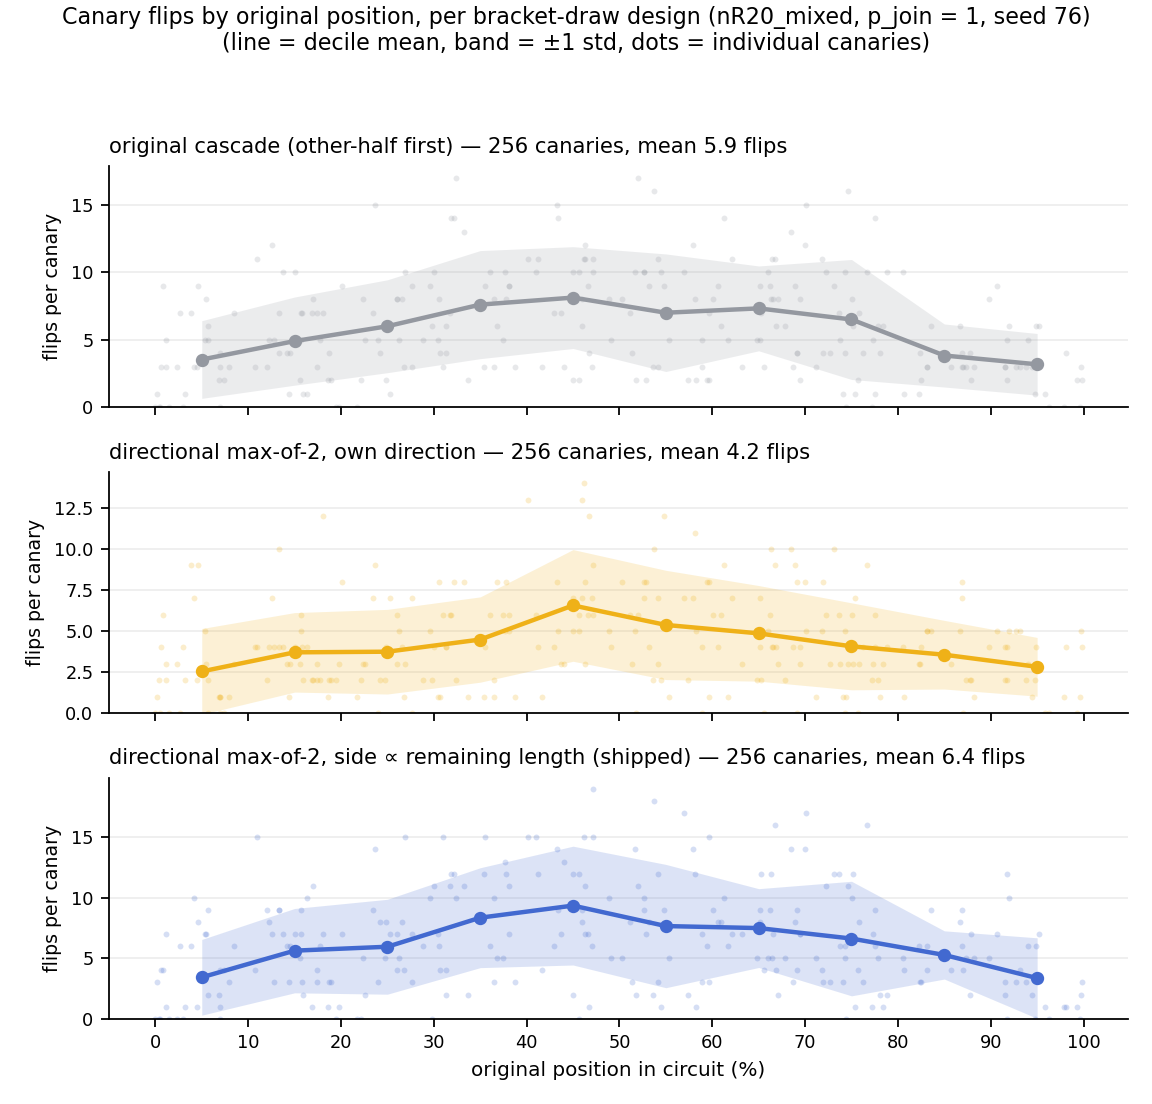
\includegraphics[width=0.92\textwidth]{../reports/split_trials_20260805/canary_flips_by_arm_nR20.png}
\caption{The Figure~1 instrument applied to the three bracket-draw arms of
Figure~\ref{fig:spans} (same input, same seed): flips per canary by original
position --- decile mean, $\pm1$ std band, individual canaries. Colors match
Figure~\ref{fig:spans}. The own-direction arm's short spans depress coverage
everywhere (mean 4.2); the cascade recovers the mid-hump (5.9) but at
near-full-circuit spans; the shipped proportional draw dominates both (6.4)
with the strongest coverage in every decile while keeping spans balanced.}
\label{fig:armcanaries}
\end{figure}

\section{Shipped parameters and launch recipe}

\begin{center}
\small
\begin{tabular}{lll}
\toprule
knob & default & meaning \\
\midrule
\texttt{--split} & off & arm the stage (forces the split twist as the only move) \\
\texttt{--split-stop} & off & end the run at the stage boundary (trial mode) \\
\texttt{--p-join} & 0.8 & probability a split carries the twist + cross (trials ran 1.0) \\
\texttt{--split-reach-k} & 2 & length bias of the bracket draw ($0$ = legacy cascade) \\
\texttt{--split-fail-limit} & 100 & exit B threshold (never approached in practice) \\
\texttt{--split-canaries} & 256 & coverage monitors, reported at the boundary \\
\bottomrule
\end{tabular}
\end{center}

Launch hygiene unchanged: export \texttt{FMIX\_STOP\_FLAG}/\texttt{FMIX\_DUMP\_FLAG},
budget \texttt{--moves} generously (the stage self-terminates; one move per
split twist, so a comfortable multiple of the \g\ count), pin every measured
knob, and keep \texttt{--p-db 0 --p-comp 0 --p-any 0} for a stage-only
invocation so no store is opened. \texttt{--split} and \texttt{--profile} are
mutually exclusive; run part 2 as its own invocation.

\section{Open items}

Part-2 calibration starts from the split form ($\times$1.7--2.0 the phase-A
size, zero comp, 50/50 CNOT/NCNOT); the thermostat target and move budget
should be sized against that, and old descent-free calibrations do not
transfer. The wide-conjunction tail of some phase-A recipes (up to $w32$)
passes through the stage untouched except for pin flips; per-gate exhaustive
verification is capped at width $<16$ (wide flips remain covered by the
global functional check). Artifacts: spec \texttt{docs/FMIX\_SPLIT\_TWIST.md},
measurements and scripts \texttt{reports/split\_trials\_20260805/}.

\end{document}
